%-------------------------------------------------------------------------------
% DEFINE THE DOCUMENT TEMPLATE (FROM SIGCOM, ACM, IEEE, ...)
%-------------------------------------------------------------------------------
\documentclass{libs/sig-alternate}

%USING SIGCOM TEMPLATE
%\documentclass[sigconf,natbib=true]{acmart}
%\settopmatter{printacmref=false} % Removes citation information below abstract
%\renewcommand\footnotetextcopyrightpermission[1]{} % removes footnote with conference information in first column
%\pagestyle{plain} % removes running headers
%-------------------------------------------------------------------------------
% PACKAGES FOR URL
%-------------------------------------------------------------------------------
\usepackage{hyperref}
\hypersetup{colorlinks, citecolor=blue, filecolor=blue, linkcolor=blue, urlcolor=blue}
%\usepackage{breakurl}
%\usepackage[hyphens]{url}

%-------------------------------------------------------------------------------
% PACKAGES AND COMMANDS FOR TABLES 
%-------------------------------------------------------------------------------
\usepackage{longtable}
\usepackage{multirow}
\usepackage{adjustbox}
\usepackage{color,colortbl,xcolor}
\usepackage{array}
\newcolumntype{L}[1]{>{\raggedright\let\newline\\\arraybackslash\hspace{0pt}}m{#1}}
\newcolumntype{C}[1]{>{\centering\let\newline\\\arraybackslash\hspace{0pt}}m{#1}}
\newcolumntype{R}[1]{>{\raggedleft\let\newline\\\arraybackslash\hspace{0pt}}m{#1}}
%-------------------------------------------------------------------------------
% PACKAGES FOR FIGURES
%-------------------------------------------------------------------------------
\usepackage{graphicx,graphics,float,subfigure,wrapfig,epstopdf}
\usepackage{dblfloatfix}%to fix the problem of [h!] [t!] [!b]
\epstopdfsetup{update}
%-------------------------------------------------------------------------------
% PACKAGES FOR REFERENCE LIST FORMAT 
%-------------------------------------------------------------------------------
\usepackage[square,numbers]{natbib}%options: round; square; curly; angle; colon; comma; authoryear; numbers; super; sort; sort&compress; longnamesfirst; sectionbib; nonamebreak;

\def\BibTeX{{\rm B\kern-.05em{\sc i\kern-.025em b}\kern-.08emT\kern-.1667em\lower.7ex\hbox{E}\kern-.125emX}} % defining the \BibTeX command - from Oren Patashnik's original BibTeX documentation.

%-------------------------------------------------------------------------------
% PACKEGE FOR CREATING GANTT VISUALIZATION (PLANNING TABLE) 
%-------------------------------------------------------------------------------
\usepackage{soul}
\usepackage{libs/gantt} %for the planning table
%-------------------------------------------------------------------------------
% CREATING COMMANDS FOR AUTOREF 
%-------------------------------------------------------------------------------
\renewcommand{\chapterautorefname }{\S}
\renewcommand{\sectionautorefname}{\S}
\renewcommand{\subsectionautorefname}{\S}
\renewcommand{\subsubsectionautorefname}{\S}
\newcommand{\subfigureautorefname}{\figureautorefname}
%-------------------------------------------------------------------------------
% CREATING COMMANDS FOR MAKING COMMENTS
%-------------------------------------------------------------------------------
\newcommand\comment[1]{{\noindent\sffamily\textbf{[COMMENT: #1]}}}
%-------------------------------------------------------------------------------
%-------------------------------------------------------------------------------
\begin{document}


%if "acmart" then the following title and keywords:
%\title{<YOUR TITLE>}
%\author{<Your Name>}
%\email{<your email>}
%\affiliation{\institution{University of Twente}}
%\maketitle
%\begin{abstract}
\comment{The structure of an abstract should have the (i) context, (ii) problem, (iii) how your proposal is different from the literature (without saying what you propose), (iv) your proposal, and (v) your most astonishing finding (or [if proposal] your expected scientific contribution(s)). Your goal is to meet $\pm$100 words. The ``context'' part describes what your reader should know to understand your research. The ``problem'' part describes why your research need to be done; why it is interesting; and why someone needs to spend time reading your work. In the ``how your proposal is different'' you should say what is the main issue in similar works that you intend to solve. The ``proposal'' part describes what your proposal and the overall methodology to achieve your proposal (goal). Finally, your ``findings'' part I recommend you to surprise your reader, make him VERY interested to read your paper. If your ``findings'' part is related to a proposal document then you should describe what do you expect (intend) to be your scientific contribution.}
\end{abstract}


%\keywords{keyword1, keyword2, keyword3, keyword4, keyword5}

\title{Title}

\numberofauthors{2} 

\author{
	\alignauthor
	Student Name\\
	\affaddr{University of Twente}\\
	\email{s-number@student.utwente.nl}
	% 2nd. author
	\alignauthor
	Jair Santanna\\
	\affaddr{University of Twente \& Northwave}\\
	\email{j.j.santanna@utwente.nl}\\
	\email{jair.santanna@northwave.nl}
}

\maketitle
%-------------------------------------------------------------------------------%
%-------------------------------------------------------------------------------
\begin{abstract}
\comment{The structure of an abstract should have the (i) context, (ii) problem, (iii) how your proposal is different from the literature (without saying what you propose), (iv) your proposal, and (v) your most astonishing finding (or [if proposal] your expected scientific contribution(s)). Your goal is to meet $\pm$100 words. The ``context'' part describes what your reader should know to understand your research. The ``problem'' part describes why your research need to be done; why it is interesting; and why someone needs to spend time reading your work. In the ``how your proposal is different'' you should say what is the main issue in similar works that you intend to solve. The ``proposal'' part describes what your proposal and the overall methodology to achieve your proposal (goal). Finally, your ``findings'' part I recommend you to surprise your reader, make him VERY interested to read your paper. If your ``findings'' part is related to a proposal document then you should describe what do you expect (intend) to be your scientific contribution.}
\end{abstract}


\section{Introduction} 
\label{sec:introduction}


\comment{The Introduction section has more or less the same structure as your abstract. The difference is that in the abstract each part is one statement/phrase, while in the introduction each part is a paragraph. So, (i) context, (ii) problem, (iii) proposal, and your most astonishing (iv) finding. Of course in the Introduction section you can give far more details than in the abstract. Avoid to copy and paste statements, re-write with different words.}

\comment{In addition to the structure that you already know you should include your \textit{research questions} between the ``proposal'' paragraph and the ``findings''. The statement that precede the RQ is something like the following: }

To pursue our goal, we have defined the following research questions (RQ) as the basis of our research: 
\begin{itemize}	
	\item \textbf{RQ1:} What are ..?
	\item \textbf{RQ2:} How to ... ?
	 \item \textbf{RQ3:} How to ...?
\end{itemize}



\comment{Please, avoid "yes or no" questions. Make questions that your reader are not able to answer immediately. Usually the questions depend on each other, it means that to answer one question you must answer the one before.}

\comment{Before a little bit of your most astonishing findings you must to introduce the structure of your paper (or proposal). Usually the text looks like the following.}
 
``The remainder of this paper (or proposal) is organized as follows. Section 2 will discuss the approaches expected for answering each research question. After that, we present a preliminary planning for the research questions in Section 3. Finally, we conclude with a proposal and planning for the thesis structure in Section 4.'' 






\section{Related Work}

Go to Google scholar and search using keywords related to your research. Then,
download some paper that the title immediately show similarities with your
research. You must be able to judge the strong and weak-points of each paper.
Also, you can extend your literature study by looking the related work section
of each downloaded paper. In addition to that, you can look who cited the papers
that you decided to include (till this moment) on your research (google scholar
shows this information for you). This step is important because the papers that
cited the paper that you decide to include on your research are potential papers
to include on your section. Note that the final goal of this section is a table
that summarizes the characteristics of each paper and your critical analysis to
highlight the existing gaps of research.

Examples of how to make a reference:
\begin{itemize}
	\item $\backslash$citep outputs: \citep{jjsantanna2015IM1}
	\item $\backslash$citet outputs: \citet{jjsantanna2015IM1}
\end{itemize}

\section{Methodologies}
<brief summary explaining the content and the connection><you could even to make a picture explaining how the parts connect for example a conceptual figure with your idea (if possible). On this, I must say that Figures MUST be in pdf format (I like to use Inkscape to create my figures, then I export to pdf) [ask me how, for help]> 

\subsection{On answering RQ1}

\subsection{On answering RQ2}

\subsection{On answering RQ3}
\begin{figure}[h!]
	\label{fig:approach}
	\centering
	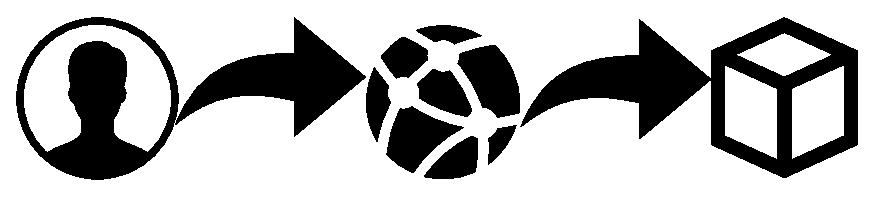
\includegraphics[width=0.45\textwidth]{figs/example.eps}
	\caption{Example of Figure.}
\end{figure}
\section{Planning}
 In this section we will shortly discuss the planning of the study. The study has been split into six parts, as can be seen in the table below. Note that a planning such as this when is to be seen as a guideline. There are however some hard deadlines for handing in drafts and final versions. Here we have an overview of the deadlines:
 \begin{itemize}	
	\item December 1st: Final proposal submission
	\item January 19th: Draft paper submission
	\item January 26th: Final paper submission
	\item January 31th: Conference presentation
\end{itemize}
The planning is made in order to adhere to these submission deadlines.

% More examples on how to do a planning table you can see in \url{http://www.martin-kumm.de/wiki/doku.php?id=05Misc:A_LaTeX_package_for_gantt_plots}

\begin{figure}[ht]
		\noindent\resizebox{0.49\textwidth}{!}{
	\begin{gantt}[xunitlength=0.5cm,fontsize=\small,titlefontsize=\small,drawledgerline=true]{15}{12} %(1)lines (2)columns
		
		\begin{ganttitle} %Month
			\titleelement{\textbf{Planning Table}}{12}
		\end{ganttitle}
		
		\begin{ganttitle} %Month
			\titleelement{November}{3}
			\titleelement{December}{5}
			\titleelement{January}{4}
		\end{ganttitle}
		\begin{ganttitle} % Week number
			\numtitle{1}{1}{12}{1}
		\end{ganttitle}
		\ganttbar[color=gray]{Proposal}{0}{3}
		\ganttmilestone[color=orange]{Draft proposal}{2}
		\ganttmilestone[color=red]{Final proposal}{3}
		\ganttbar[pattern=grid,color=orange]{Writing}{3}{8}
		\ganttbar[color=blue]{RQ1}{3}{1}
		\ganttcon{3}{3}{3}{7}
		\ganttbarcon[color=blue]{RQ2}{4}{2}
		\ganttbar[pattern=grid,color=red]{Holidays}{6}{2}
		\ganttbar[color=blue]{RQ3}{8}{2}
		\ganttcon{6}{8}{8}{10}
		\ganttbarcon[color=blue]{RQ4}{10}{1}
		\ganttmilestone[color=orange]{Draft Paper submission}{10}
		\ganttmilestone[color=red]{Final Paper submission}{11}
		\ganttbar[color=green]{Presentation}{11}{1}
		\ganttcon{11}{11}{11}{14}

	\end{gantt}	
		}
\end{figure}



% The research topics part consists solely of a literature study that focuses on ... All relevant information learned from this will be integrated in a survey that will form the first part of the thesis.

% Following the research topics are each of the research questions, with time allotted at the end of each research question to integrate the results into the thesis. 
%-------------------------------------------------------------------------------%
%-------------------------------------------------------------------------------
\newcommand{\newblock}{}
\bibliographystyle{unsrtnat} %abbrvnat OR unsrtnat OR plainnat
\bibliography{my_bibliography}
%-------------------------------------------------------------------------------%
%-------------------------------------------------------------------------------
\newpage
\section*{IMPORTANT NOTES:}
\begin{itemize}
	\item I DO recommend: \url{https://www.youtube.com/watch?v=g3dkRsTqdDA}
	\item Figures MUST be in pdf format (I like to use Inkscape to create my figures, then I export to pdf);
	\item Graphs MUST be plotted using gnuplot; 
	\item Avoid vague words: relatively, possible, ... 
	\item Avoid start with 'because'
	\item To reference something you can do like this: \cite{justyna2015SBRC}, \cite{kerkers2014aims}, \cite{jjsantanna2015IM2,jjsantanna2015IM1}, \cite{santanna2013aims} \comment{look how I did in your latex file}
	\item More examples on how to do a planning table you can see in \url{http://www.martin-kumm.de/wiki/doku.php?id=Projects:A_LaTeX_package_for_gantt_plots}
\end{itemize}

\begin{figure}[h!]
	\label{fig:approach}
	\centering
	
\includegraphics[width=0.5\textwidth]{figures/example.pdf}
	\caption{Example of Figure.}
\end{figure}

\end{document}